\input{../YKY-preamble-PPT.tex}

\usepackage{color}
\usepackage{mathtools}
\usepackage{hyperref}

%\usepackage[backend=biber,style=numeric]{biblatex}
%\bibliography{../AGI-book}
% \renewcommand*{\bibfont}{\footnotesize}

\usepackage{graphicx} % Allows including images
\usepackage{tikz-cd}
\usepackage{tikz}
\usepackage[export]{adjustbox}% http://ctan.org/pkg/adjustbox
\usepackage{verbatim} % for comments
% \usepackage{newtxtext,newtxmath}	% Times New Roman font

% \numberwithin{equation}{subsection}

\newcommand{\underdash}[1]{%
	\tikz[baseline=(toUnderline.base)]{
		\node[inner sep=1pt,outer sep=10pt] (toUnderline) {#1};
		\draw[dashed] ([yshift=-0pt]toUnderline.south west) -- ([yshift=-0pt]toUnderline.south east);
	}%
}%

\DeclareSymbolFont{symbolsC}{U}{txsyc}{m}{n}
\DeclareMathSymbol{\strictif}{\mathrel}{symbolsC}{74}

\newcommand{\highlight}[1]{\colorbox{pink}{$\displaystyle #1$}}

\newcommand{\emp}[1]{{\color{violet}\textbf{#1}}}
\newcommand*\confoundFace{$\vcenter{\hbox{\includegraphics[scale=0.2]{../2020/../confounded-face.jpg}}}$}
\newcommand{\underconst}{\includegraphics[scale=0.5]{../2020/UnderConst.png}}
\newcommand{\witness}{\scalebox{0.6}{$\blacksquare$}}
% \newcommand{\Heytingarrow}{\mathrel{-}\mathrel{\triangleright}}
\providecommand\Heytingarrow{\relbar\joinrel\mathrel{\vcenter{\hbox{\scalebox{0.75}{$\rhd$}}}}}

\begin{document}

\title{\bfseries\color{blue}{\Huge《BERT 与逻辑的结合》}}
\author{YKY} % Your name
%\institute[] % Your institution as it will appear on the bottom of every slide, may be shorthand to save space
%{
%Independent researcher, Hong Kong \\ % Your institution for the title page
%\medskip
%\textit{generic.intelligence@gmail.com} % Your email address
%}
\date{\today} % Date, can be changed to a custom date

\maketitle
\pagenumbering{gobble}

\begin{itemize}
	\item 我比较熟悉 经典逻辑 AI,写过 逻辑引擎
	\item 但我没有 BERT/GPT 的实战经验
	\item 今天我们考虑一下 结合 BERT/GPT 和 逻辑引擎 的可能,有什么优势? 
\end{itemize}

\setcounter{section}{-1}
\section{我们的策略}

\begin{itemize}
	\item 将 BERT/GPT 解释为一种 逻辑/符号演算的系统
	\item 将 逻辑结构 impose 到新的 BERT/GPT 模型 \\
		(它不再是语言模型,而是逻辑模型)
	\item 利用我们对逻辑 AI 的理解, \\
		改良这新的模型,\\
		从逻辑角度理解参数的意义
	\item 如果不这样做,BERT/GPT 仍然是 ``black box'', \\
		那就很难想出改良的思路
\end{itemize}

\section{Transformer 的 equi-variance}

\begin{equation}
\vcenter{\hbox{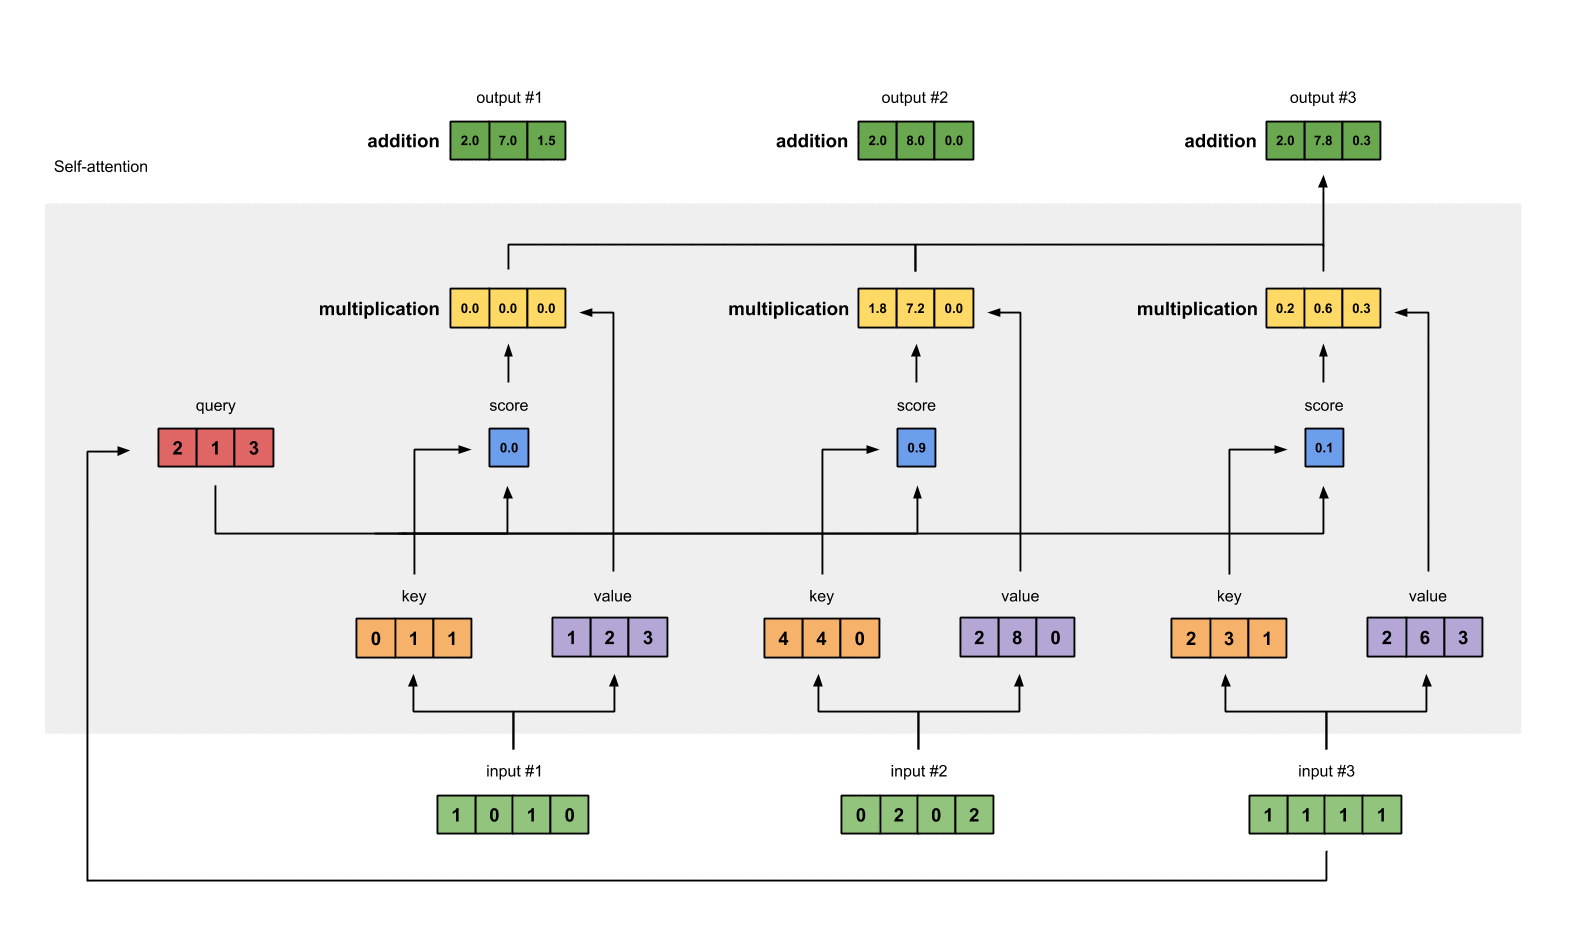
\includegraphics[scale=0.3]{self-attention.png}}}
\end{equation}

\section{Logic AI 的基本架构}

系统的 \textbf{状态} (state) = 例如: \\
\tab 我很肚饿 $\wedge$ \\
\tab 冰箱没有食物 $\wedge$ \\
\tab 现在是午夜3点 $\wedge$ \\
\tab 商店已经打烊 $\wedge$ \\
\tab .... $\wedge$ ....

换句话说,状态 是 一堆 逻辑命题 的 \textbf{集合}


\begin{itemize}
	\item 一直以来,人们觉得 大脑的 KR(knowledge representtation, 知识表述)跟符号逻辑 肯定是大相迳庭的
\end{itemize}

\section{Seq-seq-2-seq}

\begin{itemize}
	\item 逻辑 与 自然语言 之间大约有这样的对应: \\
	句子 $\approx$ 命题,词语 $\approx$ 概念,\\
	命题 = 多个概念的 concatenation
	\item 从 强化学习的角度看: \\
		状态 (state) = 命题集合,\\
		transition function: 命题集合 $\rightarrow$ 命题集合
	\item 命题集 = sequence of 命题, \\
		命题 = sequence of concepts,\\
		所以 状态 = 命题集 = sequence of sequences (seq-seq)
	\item transition fn: seq-seq $\rightarrow$ seq-seq 
		\begin{equation}
		\vcenter{\hbox{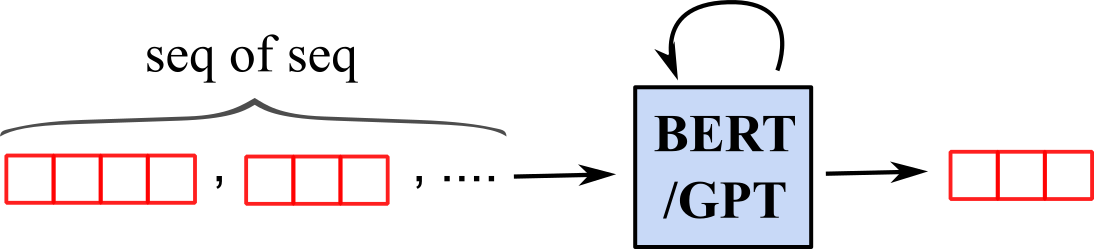
\includegraphics[scale=0.9]{seq-seq-2-seq-with-BERT.png}}}
		\end{equation}
	\item 「状态 」的另一个名称是 working memory \\
		(借用 \textbf{认知科学} 术语)
	\item 每次状态更新时,我们可以只增添一个命题,\\
		「\textbf{遗忘}」另一个命题
	\item 因此 transition fn 只需是 seq-seq $\rightarrow$ seq
	\item 而我想说的是: BERT/GPT 可能就是一种 seq-seq $\rightarrow$ seq
\end{itemize}

\section{强化学习的考虑}

\begin{itemize}
	\item 从 强化学习 的角度看,\\
	每个 iteration 要输出一个 \textbf{命题} = 几个\textbf{词语}
	\item 这 输出 对应于 强化学习的 \textbf{actions}
	\item 换句话说,每个 action = 一个命题 = 几个词语
	\item 所以,我们需要输出 在 actions 之上的 \textbf{概率分布} \\
		(而不仅仅是一个 action)
	\item 数学上 这是 $\{ \mbox{所有可能命题} \} \rightarrow \mathbb{R}$ 的空间 $= \mathbb{R}^{|X|}$
	\item 这个空间异常大,我初时觉得 没有希望在计算机上表达
	\item 但 Dr肖达 解释了一个很有效率的方法, \\
			用 矩阵乘法 将输出 由 1024维 \textbf{扩张}到 25000维:
		\begin{equation}
		\vcenter{\hbox{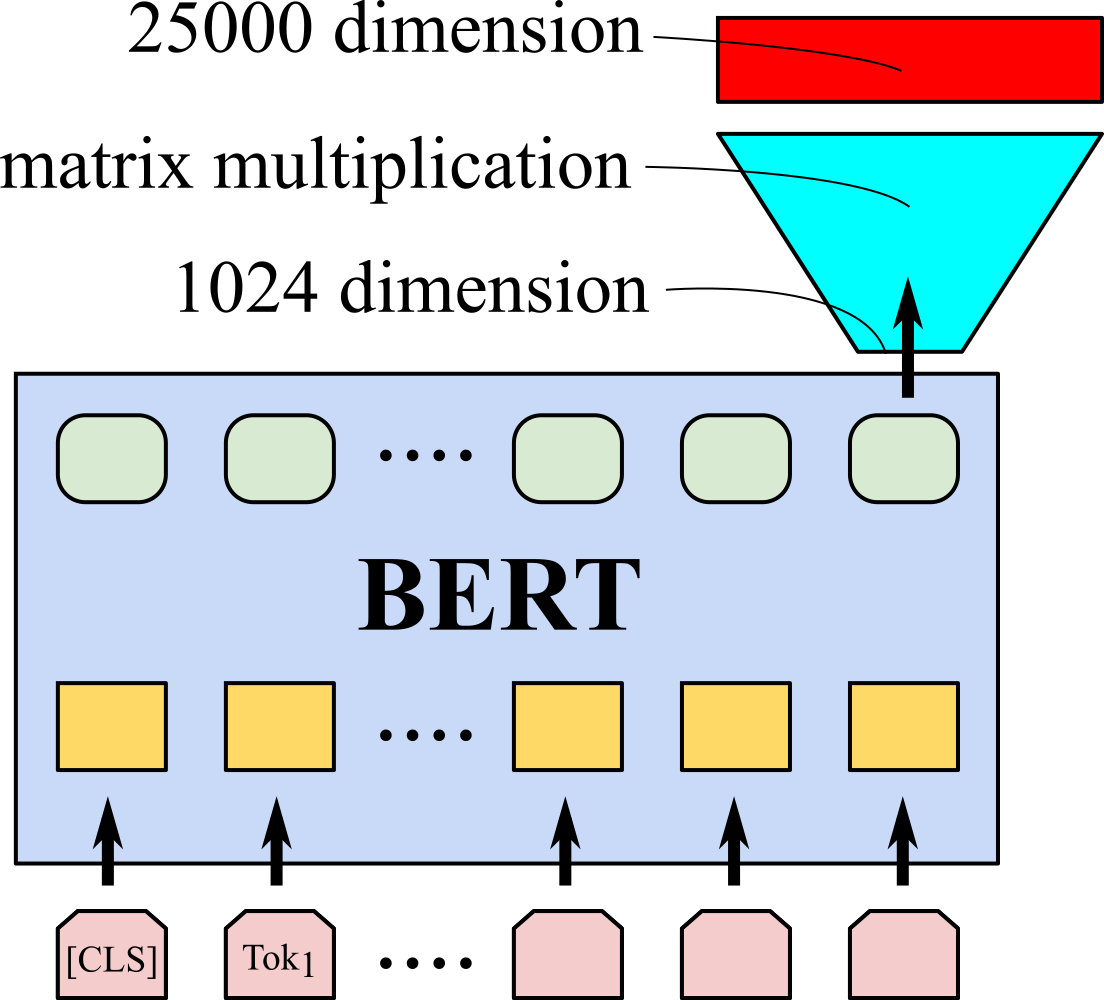
\includegraphics[scale=0.7]{BERT-action-probability-distribution.png}}}
		\end{equation}
	\item 但这个做法,其实输出的 只有 1024个 \textbf{独立}的份量
\end{itemize}

例如,「天气很热,我在家中整天\underline{\hspace*{2cm}}」\\
	\tab \textbullet 流汗 \\
	\tab \textbullet 吃冰淇淋 \\
	\tab \textbullet 喝冰水 \\
	\tab \textbullet 不穿衣服 \\
	\tab \textbullet 开冷气 ....

「女朋友说分手,我觉得\underline{\hspace*{2cm}}」\\
\tab \textbullet 很伤心 \\
\tab \textbullet 如释重负 \\
\tab \textbullet 很气愤 \\
\tab \textbullet 很妒忌 ....

「电脑的键盘没反应,可能是因为\underline{\hspace*{2cm}}」\\
\tab \textbullet 未插线 \\
\tab \textbullet 电线断了 \\
\tab \textbullet 档机了 \\
\tab \textbullet 视窗未 active ....

考虑这些例子,我暂时不清楚 1024维 够不够用。 \\
以 1024-dim 表示所有 \textbf{概念} 是足够的(cf. Word2Vec) \\
但未知它能不能够 表示所有常见的 \textbf{multi-modal} 概率分布。
% 似乎 1024 个份量,长远来说是不够的。 

\begin{comment}
\newcommand{\ttt}{$\blacktriangleright$}
那怎么解决呢? \\
有个方法是 将所有概念 按照「本体论」\textbf{ontology} 分类, \\
例如: 物体\ttt 生物\ttt 人体\ttt 上肢\ttt 手臂\ttt 手\ttt 手指 \\
\let\ttt\undefined
然后 每次输出的是一个 sub-class 的 label, \\
分多次输出,\\
而且每次输出时,\\
上一个 sub-class label 也是输入的一部分。
\end{comment}

\section{BERT/GPT 是符号演算系统}

Few-shot generalization.


\section{Relation algebra}

Relation algebra 似乎是一种更 接近 自然语言 的 逻辑形式:
\begin{equation}
\begin{tabular}{ccccc}
$F$ & $\circ$ & $F$ & = & $G$ \\
爸爸 & 的 & 爸爸 & 是 & 爷爷
\end{tabular}
\end{equation}

\section{自动 产生/运行 代码}

「计算我生命中的秒数」

% \section*{References}
% \cc{欢迎提问和讨论}{Questions, comments welcome} \smiley \\ \vspace*{0.4cm}
% \printbibliography

\end{document}
